\chapter{Xây dựng chương trình minh họa}

\section{Công nghệ sử dụng}

Chương trình minh họa được triển khai trong thư mục \texttt{Homework07/Group}. Ứng dụng là JavaFX desktop app, chạy bằng Maven và JDK 22. Tầng lưu trữ thật dùng Supabase REST API; tầng test dùng \ucname{InMemoryStore} để kiểm thử nhanh và không phụ thuộc mạng.

\begin{longtblr}{
  width = \textwidth,
  colspec = {Q[0.24\textwidth, l] Q[0.26\textwidth, l] X[l]},
  hlines,
  vlines,
  rowhead = 1,
  row{1} = {font=\bfseries},
}
Nhóm công nghệ & Công nghệ & Vai trò \\
Ngôn ngữ và runtime & JDK 22 & Biên dịch và chạy ứng dụng; cấu hình Maven đặt \texttt{maven.compiler.release=22}. \\
Quản lý build & Maven 3.9+ & Chạy build, test, package và JavaFX app. \\
Giao diện & JavaFX 22.0.2 & Xây dựng màn hình đăng nhập, dashboard và các màn hình nghiệp vụ. \\
Kiểm thử & JUnit Jupiter 5.10.3 & Viết unit/integration test cho domain rule, facade, Supabase adapter và ma trận tính năng. \\
Lưu trữ thật & Supabase REST & Lưu request, Site, tồn kho, allocation plan, order, receipt, user và log. \\
Lưu trữ kiểm thử & \ucname{InMemoryStore} & Chạy test tự động không cần Supabase thật. \\
\end{longtblr}

\section{Cấu trúc thư mục}

\begin{longtblr}{
  width = \textwidth,
  colspec = {Q[0.36\textwidth, l] X[l]},
  hlines,
  vlines,
  rowhead = 1,
  row{1} = {font=\bfseries},
}
Thư mục/package & Nội dung chính \\
\pathtext{src/main/java/vn/edu/hust/itss/group15/app} & JavaFX entrypoint, session và wiring giao diện. \\
\pathtext{app/ui} & Các màn hình \ucname{LoginView}, \ucname{DashboardView}, \ucname{RequestView}, \ucname{SiteView}, \ucname{InventoryView}, \ucname{AllocationView}, \ucname{OrderView}, \ucname{ReceivingView}, \ucname{AdminView}. \\
\pathtext{application} & Service theo use case: import request, Site, inventory, allocation, order, receipt, admin, auth và \ucname{ImportOrderingFacade}. \\
\pathtext{domain} & Entity, enum, record và rule nghiệp vụ thuần như \ucname{AllocationPolicy}. \\
\pathtext{application/port} & Interface \ucname{Store}, tách tầng application khỏi chi tiết lưu trữ. \\
\pathtext{infrastructure/persistence/supabase} & Adapter Supabase REST, cấu hình môi trường và JSON mapping. \\
\pathtext{infrastructure/persistence/memory} & Adapter bộ nhớ phục vụ test. \\
\pathtext{src/main/resources/db/schema.sql} & SQL tạo bảng Supabase. \\
\pathtext{src/test/java} & JUnit tests cho chính sách phân bổ, facade, bảo mật mật khẩu, Supabase adapter và ma trận tính năng. \\
\end{longtblr}

\section{Sơ đồ dịch chuyển màn hình}

Ứng dụng bắt đầu tại màn hình đăng nhập. Sau khi đăng nhập, dashboard hiển thị thanh điều hướng trái và mở các màn hình theo quyền của người dùng. \actorname{SystemAdministrator} truy cập được toàn bộ màn hình, các vai trò nghiệp vụ chỉ truy cập nhóm chức năng liên quan.

\diagramfigure{diagram/overview/ClassDiagram_1_000.png}{Sơ đồ chuyển đổi màn hình tổng quan.}{fig:build-screen-transition-overview}

\begin{figure}[H]
  \centering
  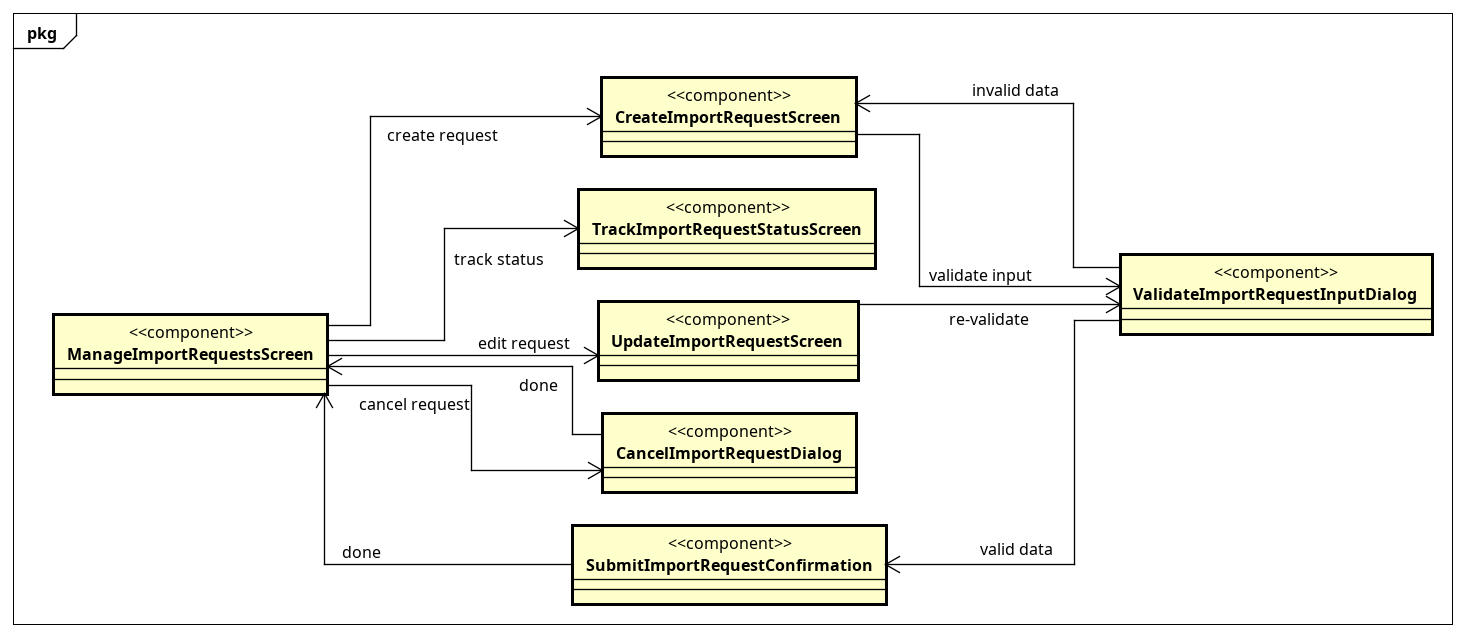
\includegraphics[width=0.48\textwidth,height=0.32\textheight,keepaspectratio]{diagram/UC001_ManageImportRequests_all/ClassDiagram_6_000.png}
  
\includegraphics[width=0.48\textwidth,height=0.32\textheight,keepaspectratio]{diagram/UC004_PlanImportAllocation_all/ClassDiagram_6_000.png}
  \caption{Ví dụ sơ đồ chuyển màn hình theo use case.}
  \label{fig:build-screen-transition-samples}
\end{figure}

\section{Giao diện minh họa}

Các hình dưới đây minh họa giao diện JavaFX theo cấu trúc màn hình thật của chương trình. Ảnh được dựng từ dữ liệu demo tương ứng với \ucname{InMemoryStore} để không phụ thuộc Supabase thật khi biên soạn báo cáo.

\begin{figure}[H]
  \centering
  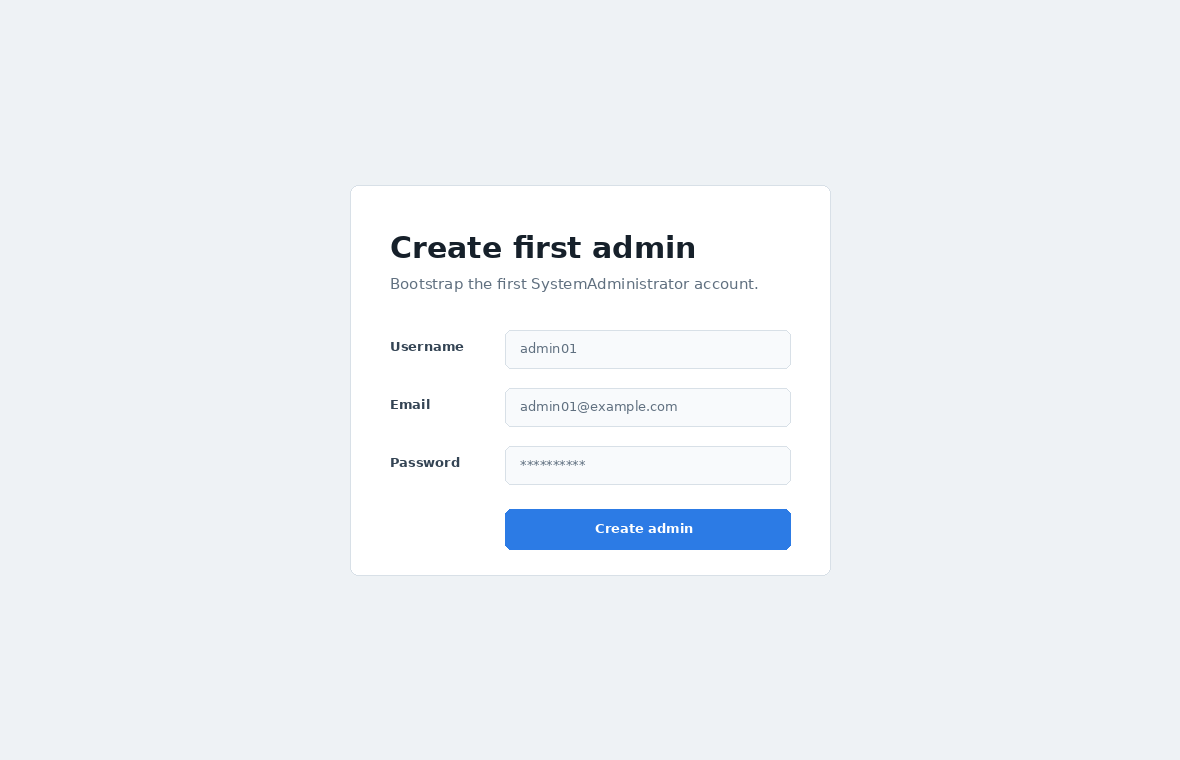
\includegraphics[width=0.92\textwidth,height=0.60\textheight,keepaspectratio]{screenshots/login.png}
  \caption{Màn hình tạo tài khoản quản trị đầu tiên.}
  \label{fig:ui-login}
\end{figure}

\begin{figure}[H]
  \centering
  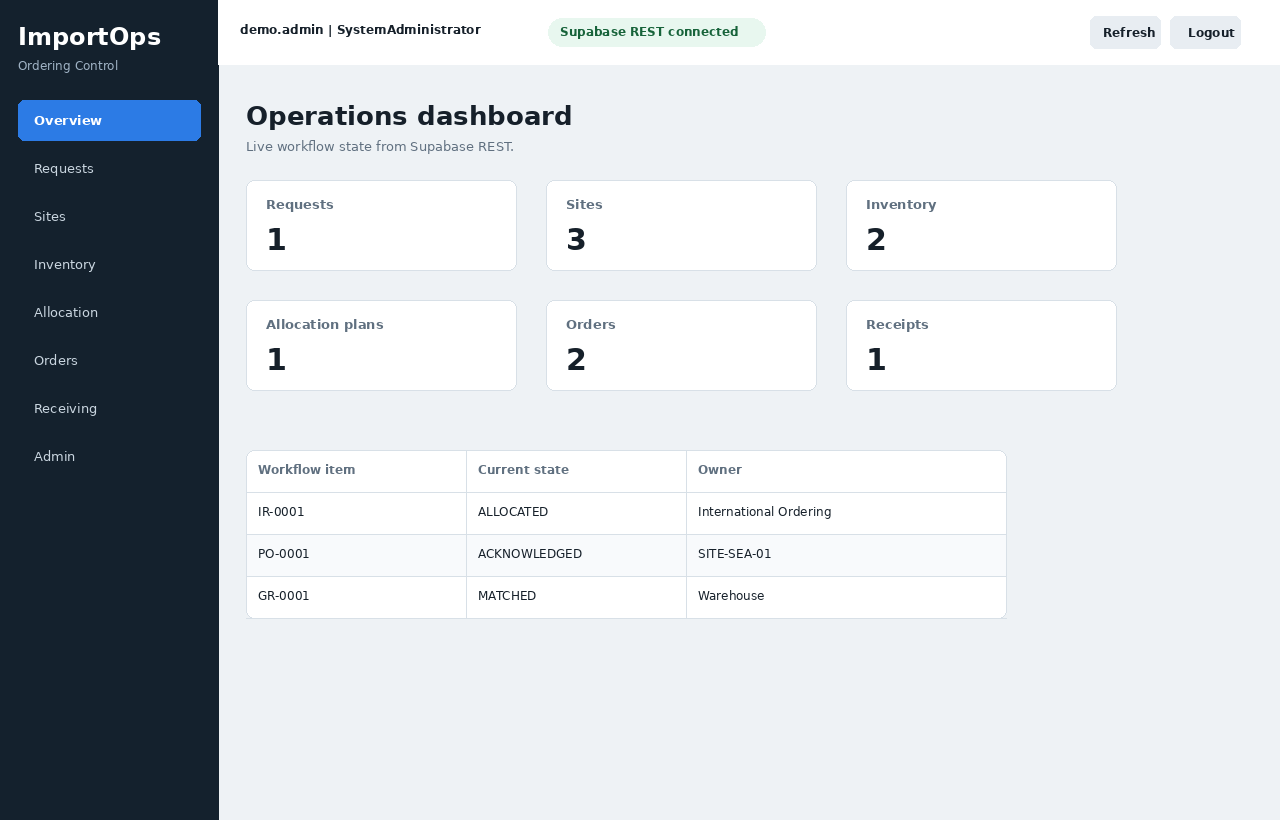
\includegraphics[width=0.92\textwidth,height=0.60\textheight,keepaspectratio]{screenshots/overview.png}
  \caption{Dashboard tổng quan vận hành.}
  \label{fig:ui-overview}
\end{figure}

\begin{figure}[H]
  \centering
  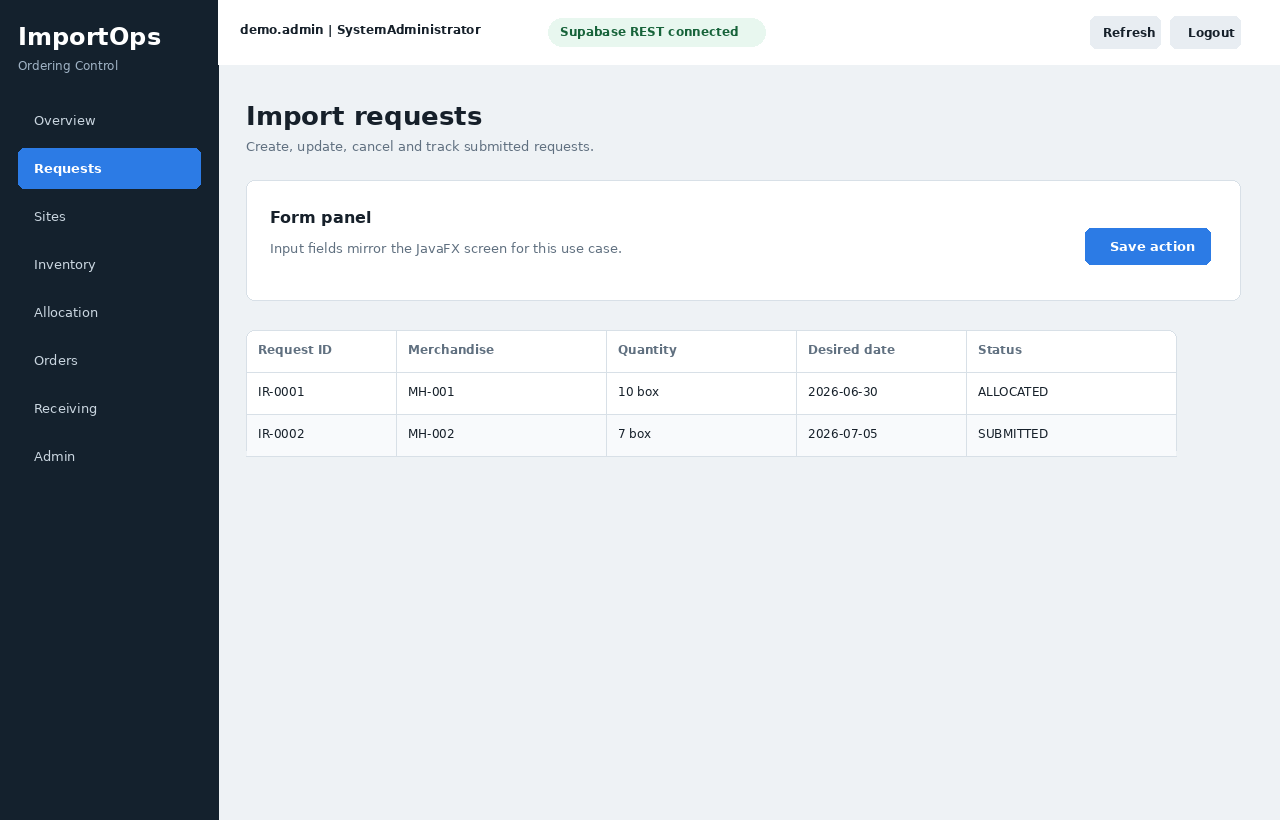
\includegraphics[width=0.48\textwidth,height=0.33\textheight,keepaspectratio]{screenshots/requests.png}
  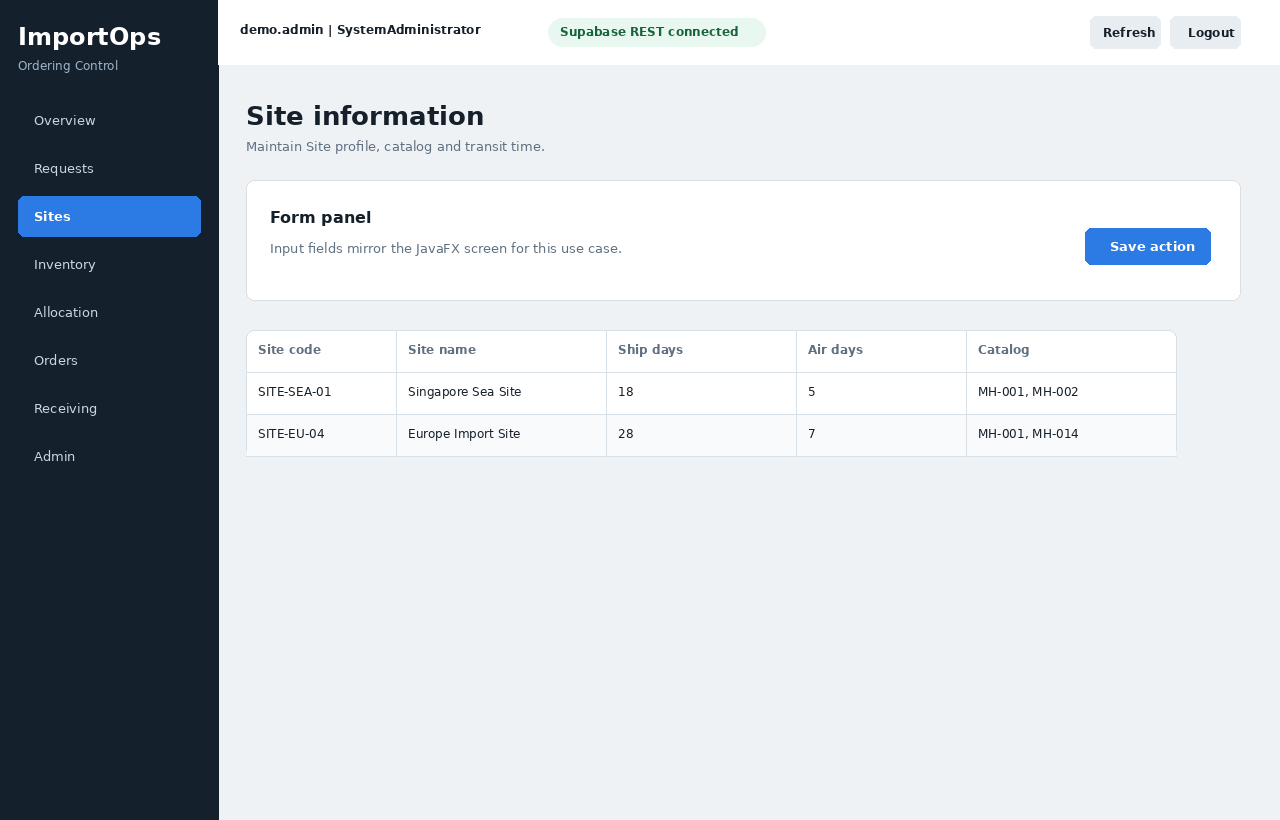
\includegraphics[width=0.48\textwidth,height=0.33\textheight,keepaspectratio]{screenshots/sites.png}
  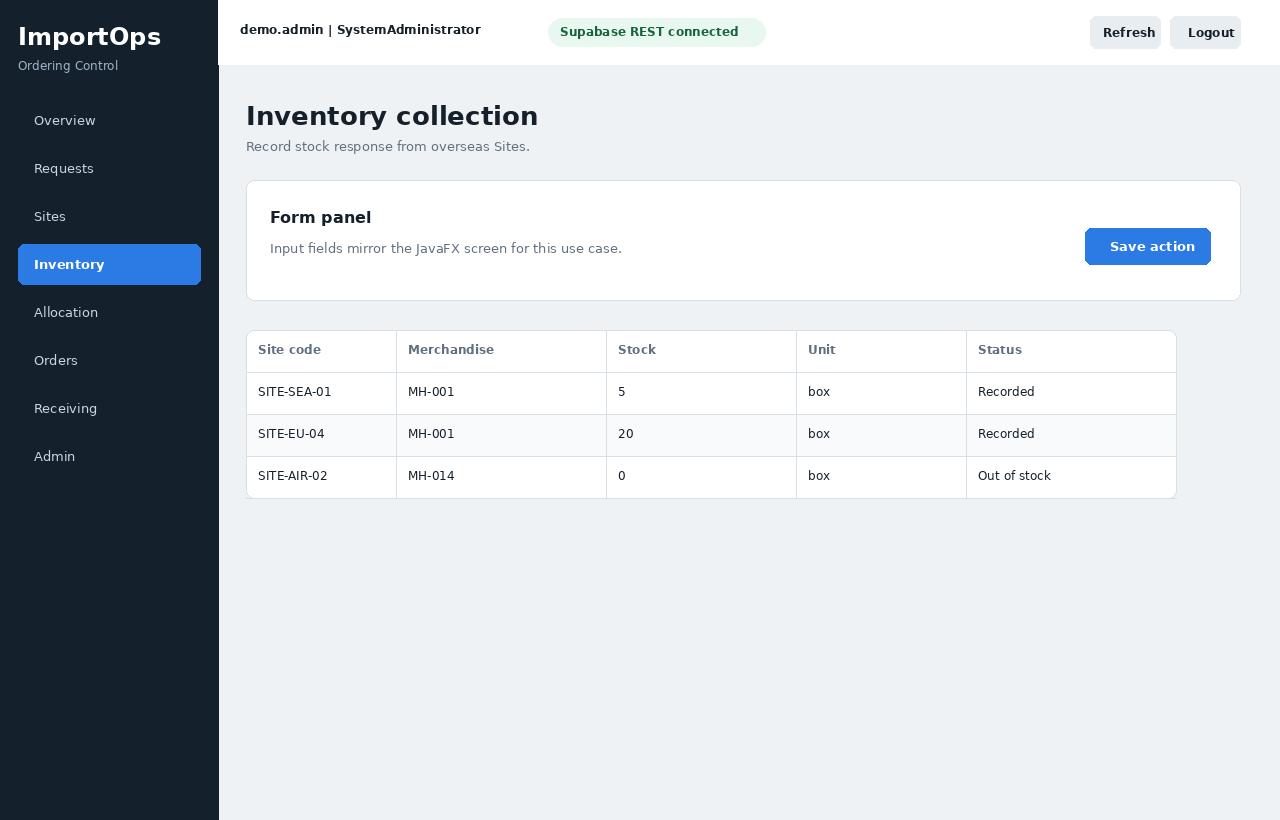
\includegraphics[width=0.48\textwidth,height=0.33\textheight,keepaspectratio]{screenshots/inventory.png}
  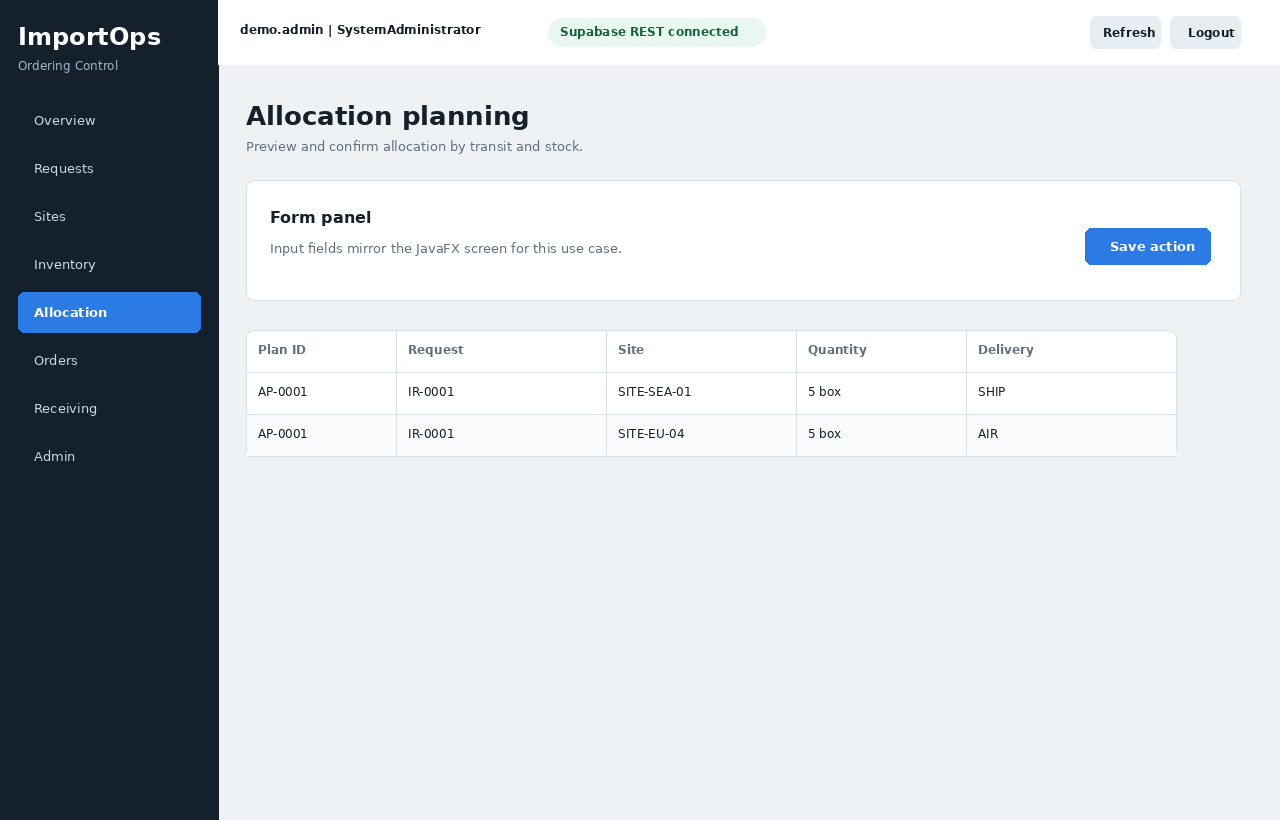
\includegraphics[width=0.48\textwidth,height=0.33\textheight,keepaspectratio]{screenshots/allocation.png}
  \caption{Các màn hình tạo yêu cầu nhập, quản lý Site, thu thập tồn kho và lập phân bổ.}
  \label{fig:ui-core-flow-1}
\end{figure}

\begin{figure}[H]
  \centering
  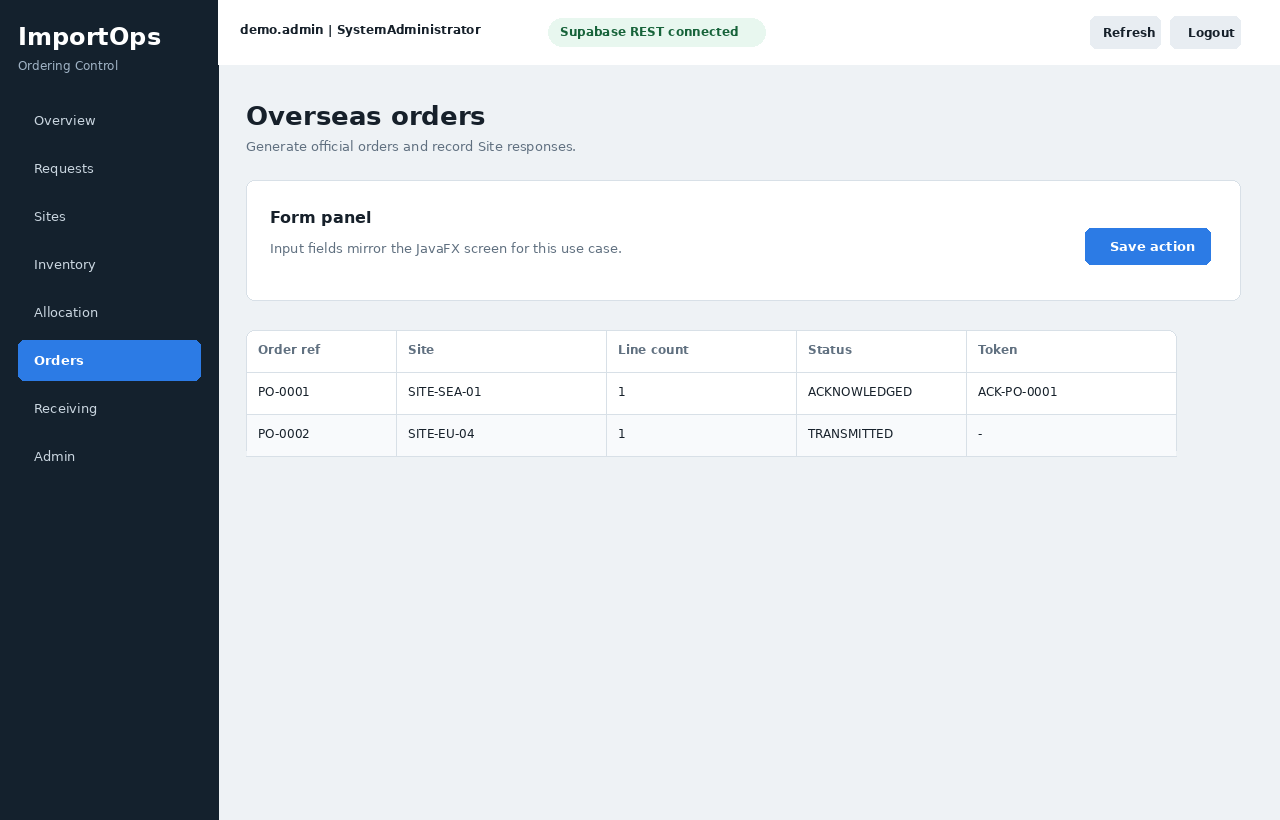
\includegraphics[width=0.48\textwidth,height=0.33\textheight,keepaspectratio]{screenshots/orders.png}
  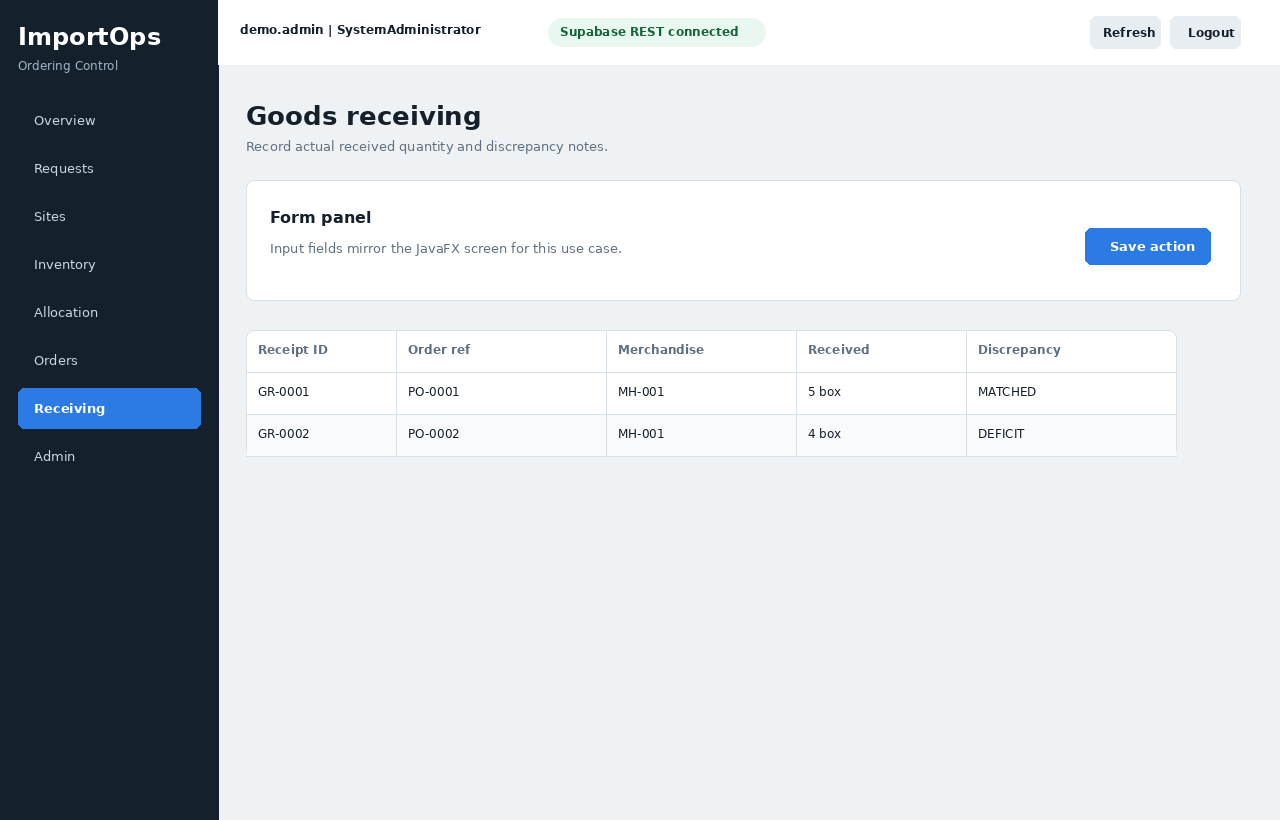
\includegraphics[width=0.48\textwidth,height=0.33\textheight,keepaspectratio]{screenshots/receiving.png}
  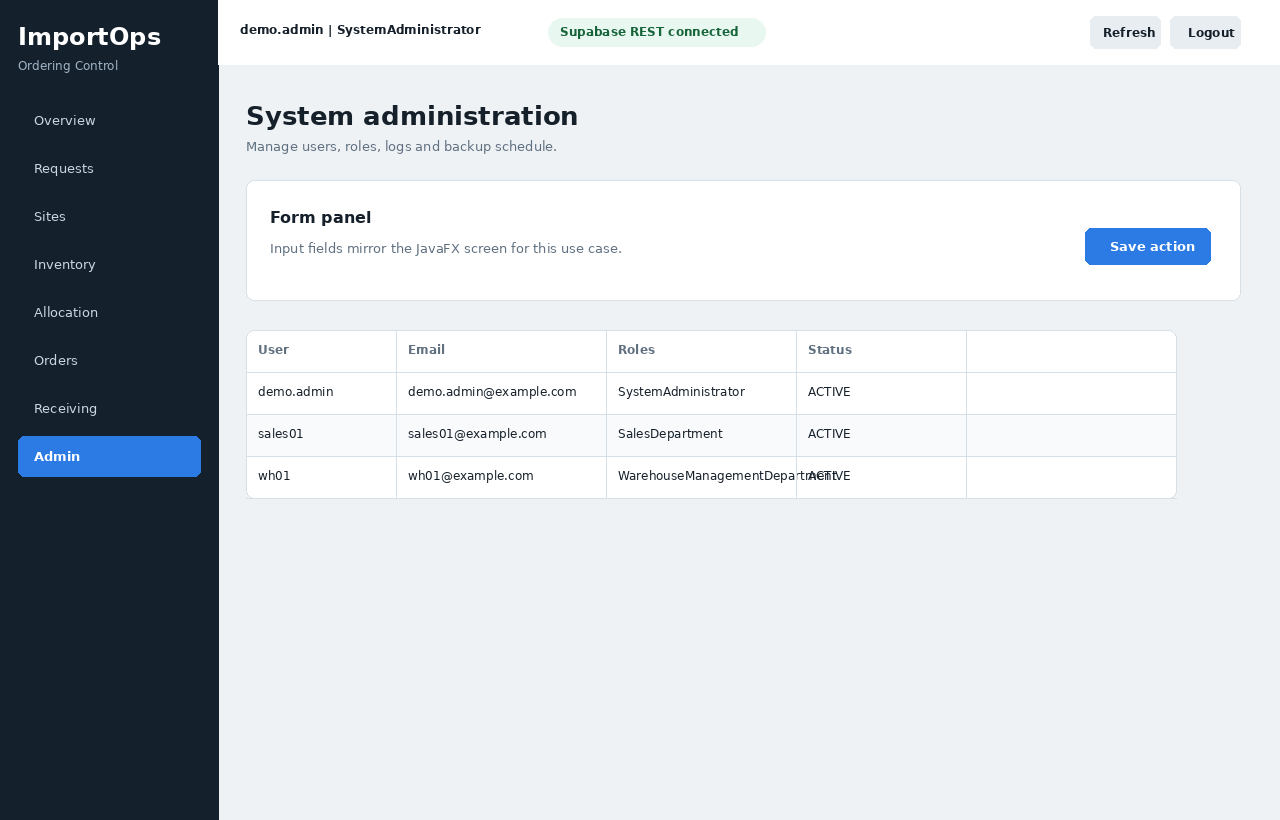
\includegraphics[width=0.48\textwidth,height=0.33\textheight,keepaspectratio]{screenshots/admin.png}
  \caption{Các màn hình đặt hàng, nhận hàng và quản trị hệ thống.}
  \label{fig:ui-core-flow-2}
\end{figure}
